\section{Implementacja}

\subsection{Plan implementacji}

Szczegółowe fazy implementacji projektu prezentują się w następujący sposób:

\begin{enumerate}
	\item [1.] Przygotowanie bazy wzorców	
	\begin{itemize}	
		\item Podział nagranych słów na odcinki czasowe o długości 0,05s
		\item Ekstrakcja parametrów słów wzorcowych poprzez FFT oraz bank filtrów
		\item Sprawdzenie powtarzalności wyników dla tego samego słowa, czyli przydatności algorytmu
	\end{itemize}

	\item [2.] Przetestowanie skuteczności programu
	\begin{itemize}	
		\item Nagranie zdań, w których pojawiają się słowa takie, jak w bazie wzorców oraz dodatkowe
		\item Ekstrakcja parametrów dla odcinków zdań i obliczenie korelacji między nimi i słowami wzorcowymi
		\item Wynik: fragmenty, dla których współczynnik korelacji jest większy od zadanego progu zostają uznane za znalezione słowa.
	\end{itemize}
\end{enumerate}

Poszczególne etapy zostały dokładnie opisane w kolejnych punktach dokumentu.


\subsection{Baza wzorców}

Na początku należało wyznaczyć słowa, które mają być wyszukiwane w nagraniach. W tym przypadku zdecydowano się na następujące: ,,książka``, ,,krzesło`` oraz ,,fotel``. \\
Przy gromadzeniu nagrań został uwzględniony fakt, że dla różnych osób rejestrowane parametry dźwięków mogą się różnić. Dlatego swego głosu do celów badawczych udzieliły osoby różnej płci. Ostatecznie w bazie znalazły się trzy słowa nagrane przez trzy osoby, po dziewięć razy każde, a więc jeden wyraz został powtórzony 27 razy.


\subsection{Ekstrakcja parametrów}

Po podzieleniu nagranych słów na odcinki odpowiedniej długości poddano je działaniu kilku algorytmów. Pierwszy z nich to szybka transformata Fouriera o 128-miu punktach, a konkretnie część rzeczywista tej transformaty. \\
Dla tak przetworzonych danych można było zastosować bank filtrów. Dla potrzeb projektu wybrano zestaw składający się z 10-ciu filtrów trójkątnych w skali melowej. Ekstrakcji dokonano w zakresie 160-6600 Hz. Dane powstałe w wyniku operacji związanych z FFT przemnożono przez stworzony w ten sposób filtr. Na ilustracji \ref{rys:fftFiltry}. zobrazowano relację, jaka występuje pomiędzy tymi danymi. \\
W wyniku powyższych działań dla każdego słowa otrzymano macierz parametrów (po jednym wektorze dla odcinka czasowego).

\begin{figure}[H]
	\centering
	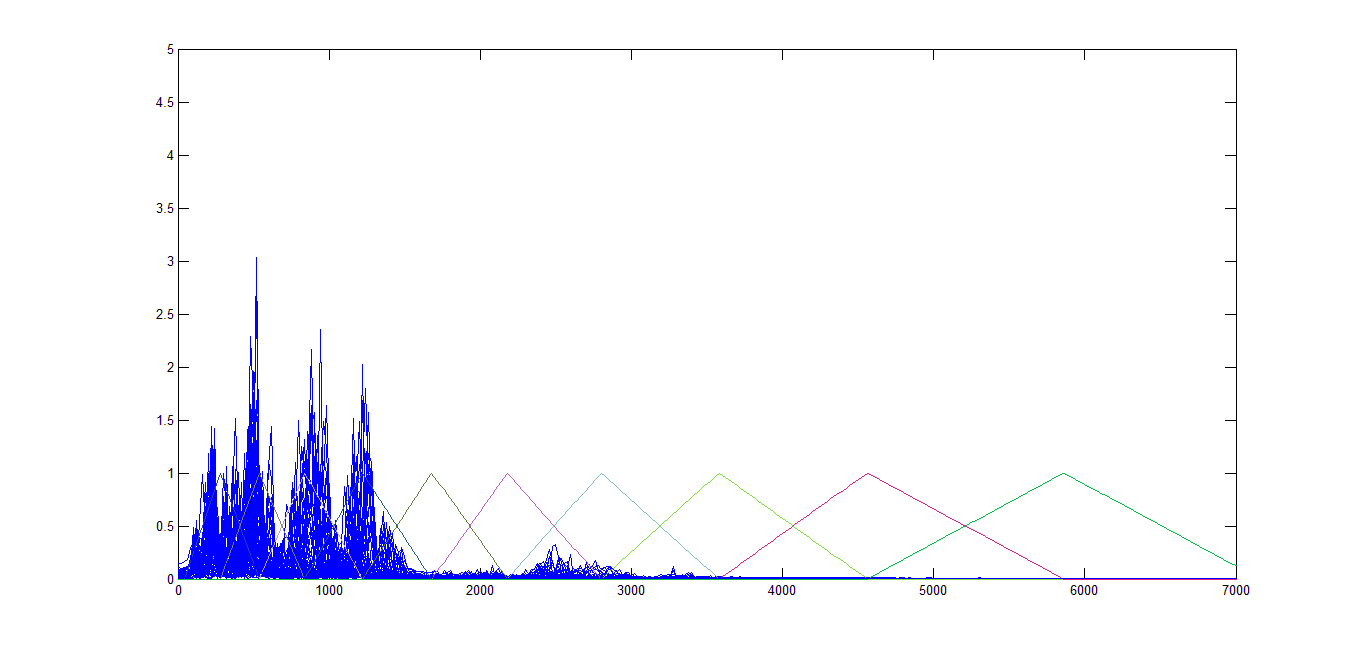
\includegraphics[scale=0.5]{fftFiltersBank}
	\caption{Wynik FFT z nałożonym bankiem filtrów}
	\label{rys:fftFiltry}
\end{figure}


\subsection{Sprawdzenie powtarzalności wyników}

Analizowanie i porównanie wartości otrzymanych parametrów liczbowych może być czasochłonne. W związku z tym, by szybko otrzymać poglądowe wyniki podobieństw pomiędzy kolejnymi nagraniami słowa, wykorzystano mapę kolorów (dany kolor odpowiada określonej liczbie). Dzięki niej można obejrzeć naraz wszystkie wyniki i ocenić, jak bardzo są do siebie podobne. Na rysunku \ref{rys:fotel_param} pokazano takie mapy dla słowa ,,fotel``. Nasuwa się tutaj kilka wniosków:

\begin{itemize}
	\item Macierze nie zawsze są tej samej długości
	\item Na wszystkich mapach powtarza się kilka miejsc
	\item Obserwując kolory można zauważyć tendencję do określonych wyników, lecz nie są one jednakowe.
\end{itemize}

Wprawdzie przedstawione mapy prezentują wybrane słowo wypowiedziane przez jedną osobę, ale to nie znaczy, że wypowiadała je tak samo. Ważną rolę gra tutaj intonacja, szybkość mówienia czy głośność. Niemniej jednak takie właśnie wypowiedzenia powinien rozpoznawać program - różne. Dlatego jest lepiej, kiedy baza wzorców jest choć trochę zróżnicowana.

\begin{figure}[H]
	\centering
	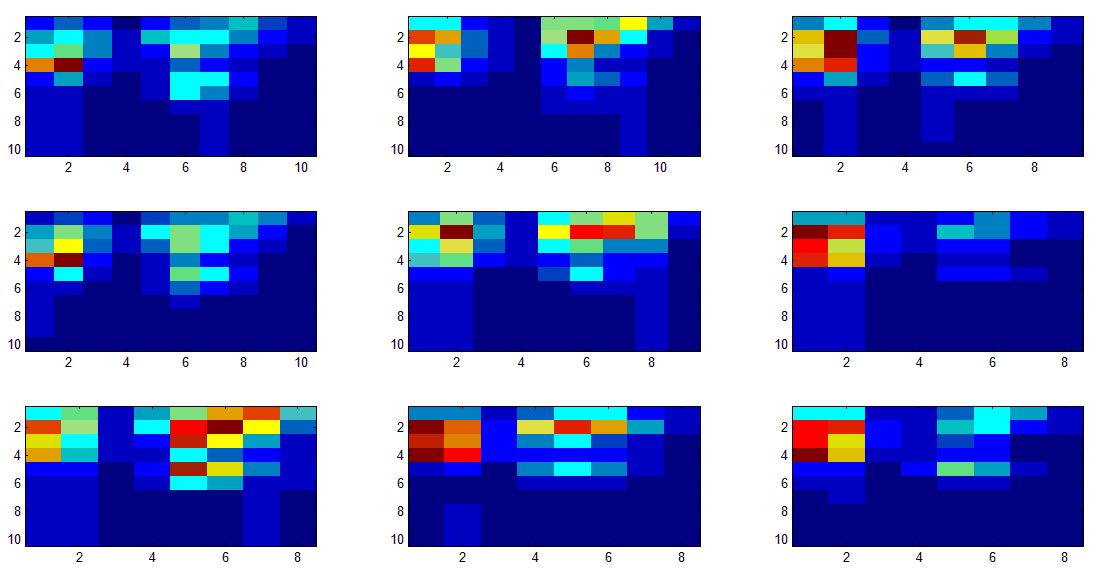
\includegraphics[scale=0.5]{fotel_param}
	\caption{Wartości dla kolejnych powtórzeń słowa ,,fotel`` przedstawione za pomocą kolorów}
	\label{rys:fotel_param}
\end{figure}

Dodatkowo wygenerowana zastała macierz autokorelacji pomiędzy zapisanymi wzorcami tego samego słowa, pozwala w sposób numeryczny określić powtarzalność parametrów, a zatem  ich przydatności przy rozpoznawania słowa w tekście.

\begin{table}[H]
	\begin{center}
\begin{tabular}{ccccccccc}
	1.0000  &  0.7569  &  0.8986  &  0.6967  &  0.9291  &  0.8563  &  0.9430  &  0.7326  &  0.9471 \\
	0.7569  &  1.0000  &  0.6380  &  0.2784  &  0.8561  &  0.5085  &  0.7421  &  0.3981  &  0.8139 \\
	0.8986  &  0.6380  &  1.0000  &  0.8246  &  0.8710  &  0.9142  &  0.8379  &  0.8551  &  0.9038 \\
	0.6967  &  0.2784  &  0.8246  &  1.0000  &  0.5785  &  0.8809  &  0.6850  &  0.9138  &  0.6520 \\
	0.9291  &  0.8561  &  0.8710  &  0.5785  &  1.0000  &  0.8092  &  0.8585  &  0.6570  &  0.9260 \\
	0.8563  &  0.5085  &  0.9142  &  0.8809  &  0.8092  &  1.0000  &  0.7629  &  0.8996  &  0.8141 \\
	0.9430  &  0.7421  &  0.8379  &  0.6850  &  0.8585  &  0.7629  &  1.0000  &  0.6992  &  0.9130 \\
	0.7326  &  0.3981  &  0.8551  &  0.9138  &  0.6570  &  0.8996  &  0.6992  &  1.0000  &  0.7081 \\
	0.9471  &  0.8139  &  0.9038  &  0.6520  &  0.9260  &  0.8141  &  0.9130  &  0.7081  &  1.0000 
\end{tabular} 
	\end{center}
	\caption{Korelacja pomiędzy powtórzeniami słowa ,,książka``}
	\label{ControlTable}
\end{table}

Na podstawie wygenerowanych \textit{heatmap} oraz macierzy korelacji, parametry poszczególnych słów uznane zostały za powtarzalne i tym samym możliwe do detekcji w nagraniu na podstawie wartości wzorcowych.

\newpage
 
\section{Testowanie skuteczności programu}

Nagrania testowe - czyli te, w których należy szukać wybranych słów - to wypowiedziane zdania zawierające co najmniej jeden z szukanych wyrazów. Zostały one poddane działaniom dokładnie takich samych algorytmów, jak wzorce. Po tych obliczeniach należy wyliczyć współczynnik korelacji między poszczególnymi fragmentami nagrań testowych a wzorcami. Jeśli otrzymana wartość jest większa od ustalonego progu (w projekcie została wykorzystana wartość 0,85) - słowo zostało znalezione. 